\documentclass{beamer}
\usepackage[T1]{fontenc}
\usepackage[utf8]{inputenc}
\usepackage{lmodern}
\usepackage{textcomp}
\usepackage{lastpage}
\usepackage{adjustbox}
%
\title{Towards Socially Responsible AI: Cognitive Bias-Aware Multi-Objective Learning
}
%
\begin{document}
\normalsize
\maketitle
%
\begin{frame}{Introduction}
%
\begin{itemize}
\item
Throughout the course of history, human society has witnessed the `us vs. them' conflict,
\item
where certain sections of the society have exhibited bias (in the form of hatred, prejudices, repression and even violence) towards other communities. >, e.g. men are more likely to be computer programmers while women are more likely to be home-makers. However, understanding which features or their combinations could lead to ethically correct responses for a particular task is not always easy, unless such a bias resurfaces out from the data and is actually observed, e.g., it is difficult to see what features (term weighting functions) could implicitly lead to the observation about female actors in Figure <ref> (right), which is nothing short of `body shaming'. >, or
\item
  * Neutralizing bias in the training data itself <cit. Specifically, we employ a multi-objective learning approach, where the intention is to increase the social acceptability (fairness) of the predicted outputs without causing a significant degradation in the effectiveness of the primary classification task (correctness).
\end{itemize}
\end{frame}
%
\begin{frame}{Introduction}
%
\begin{figure}[t]
    \centering
    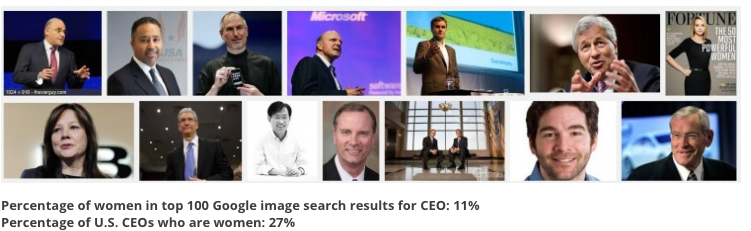
\includegraphics[width=.75\columnwidth]{ceo.png}
    
\includegraphics[width=.24\columnwidth]{qc.png}
    \caption{Examples of social bias in existing AI systems: `Google Image Search' under-representing women as CEOs (left), and `Google query completion' prioritizing \emph{appearance} over \emph{filmography} for a popular female actor (right).}
    \label{fig:bias-in-existing-AI-tools}
\end{figure}
\end{frame}
%
\begin{frame}{Related Work}
%
\begin{itemize}
\item
Demonstrating social bias in classification tasks. > demonstrated racial bias in four different tweet data sets used for hate and abusive language detection. > proposed an evaluation methodology to measure gender bias in machine translation (MT) systems and also released a dataset to support further investigation in MT bias. > proposed another approach to obtain debiased  word embedding by preserving the gender information with additional dimensions, the presence of non-zero components along which indicates gender inclined words. They removed race, gender and racial bias from existing word vectors.
\end{itemize}
\end{frame}
%
\begin{frame}{Bias-Aware Predictions}
%
\begin{itemize}
\item
Primary classification task. A model, such as the one represented in Equation <ref> can lead to socially unacceptable responses. To quantify bias formally, we define a set of categorical attributes, akin to social identity, against which a specific subset of predicted output categories may exhibit socially unacceptable biases. For an identity attribute `gender',
\item
C_gender={male, female}, if the primary task is to predict emotion from one of P={fear,anger}, then an example of cognitive bias results by defining
\item
P_s={fear} and U_gender={female} (women are prone to be more afraid than men). Using the bias response variables of Equation <ref>, the next step is then to learn a function mapping from input vectors, their associated primary task labels along with the corresponding indicator pseudo-variables for bias detection (as per Equation <ref>), (x⃗, y, y^B_i), to
\item
a Bernoulli probability distribution indicating the probability of presence (or absence) of social bias corresponding to the i-th identity attribute.
\end{itemize}
\end{frame}
%
\begin{frame}{Bias-Aware Predictions}
%
\begin{figure}[t]
    \centering
    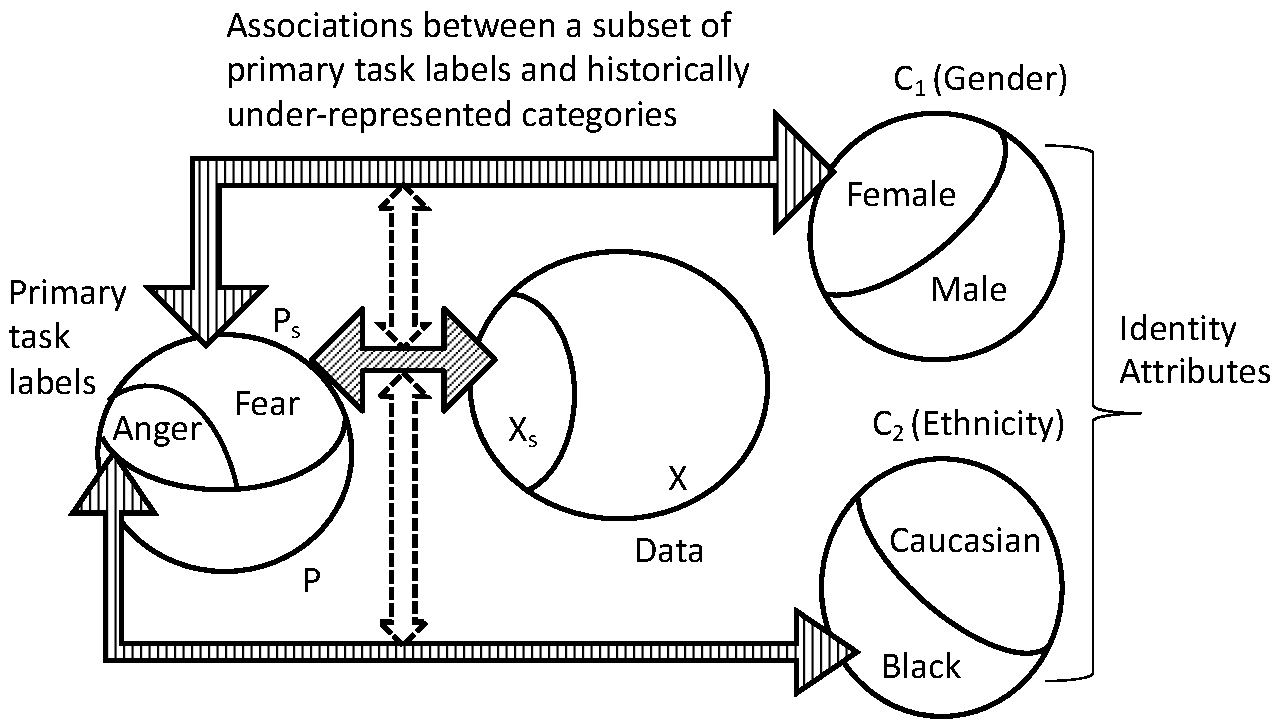
\includegraphics[width=.8\columnwidth]{bias-schematic.pdf}
    \caption{Schematic of cognitive bias removal.}
    \label{fig:schematic-bias}
\end{figure}
\end{frame}
%
\begin{frame}{Bias-Aware Predictions}
%
\begin{figure}[t]
    \centering
    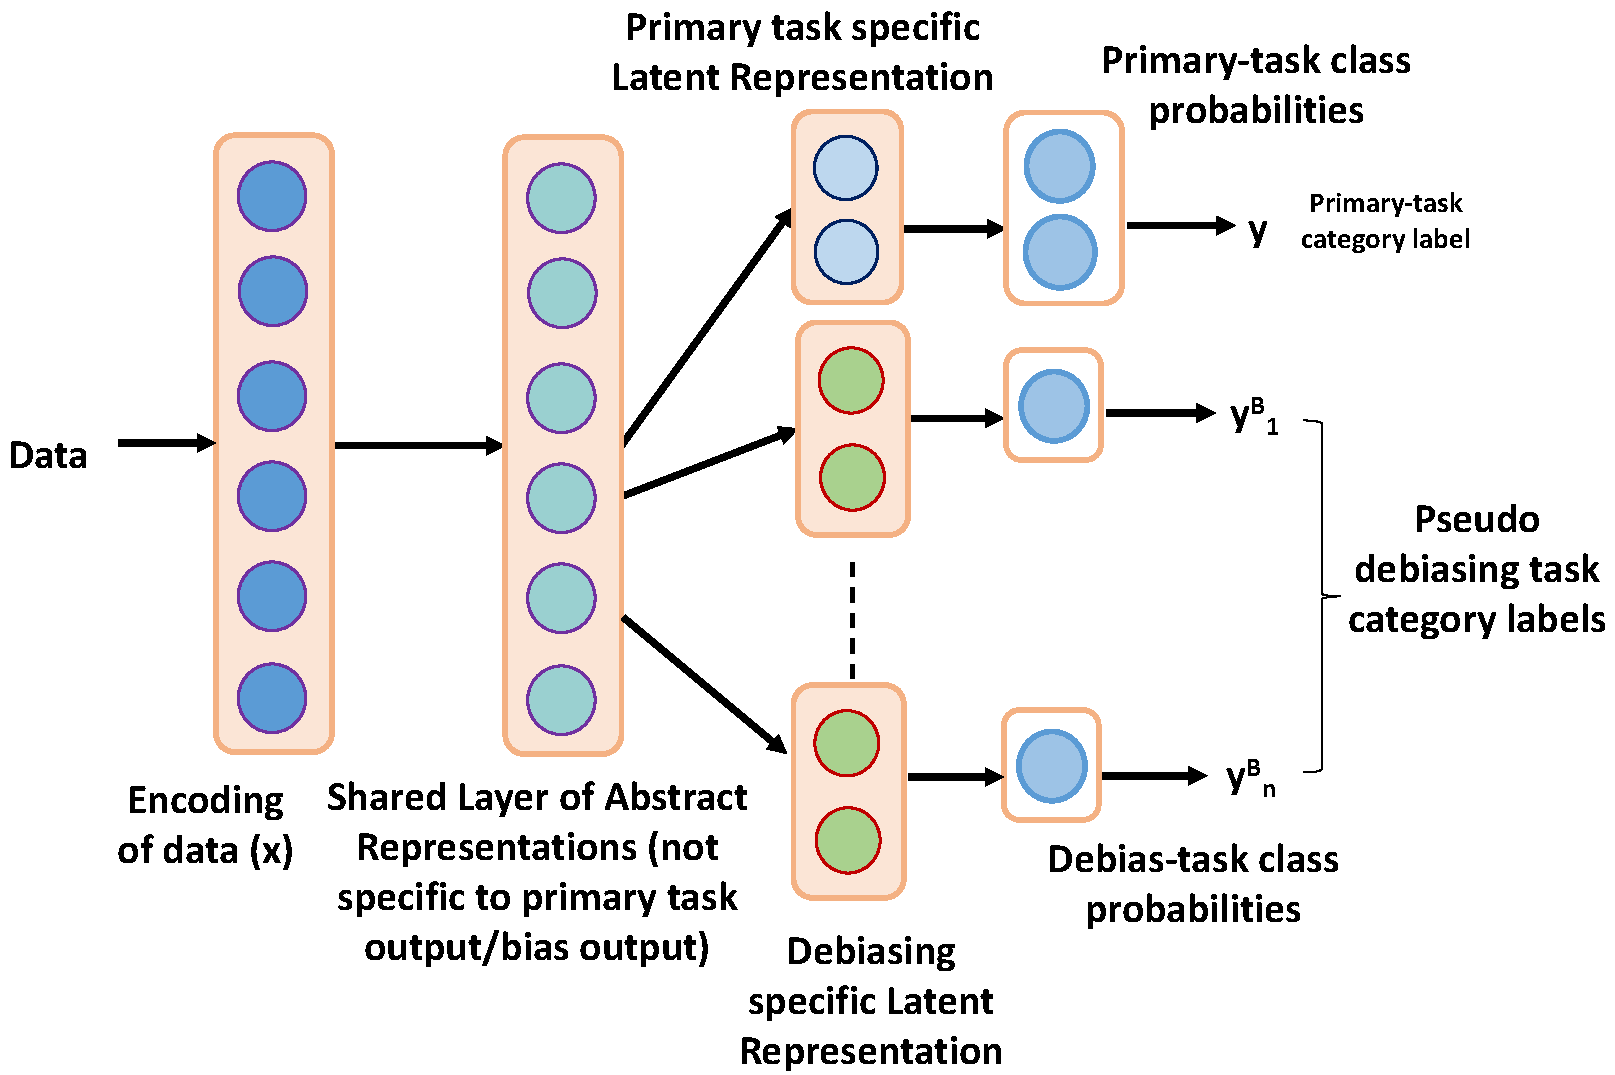
\includegraphics[width=.85\columnwidth]{debias-architecture.pdf}
    \caption{Schematic diagram of a neural network architecture for \emph{jointly} learning the primary task objective (for effective prediction) and a set of debiasing tasks (for reducing the cognitive bias in these predictions).}
\label{fig:deBiasArch}
\end{figure}
\end{frame}
%
\begin{frame}{Bias-Aware Predictions}
%
\begin{table}[t]
\adjustbox{max height=\textheight, max width=\textwidth}{
    \centering
    \small
    \begin{tabularx}{\columnwidth}{@{}l@{~~}X@{}}
    \toprule
    $\{(\vec{x}, y(\vec{x}))\}_{j=1}^{M}$ & $M$ pairs of data and primary task labels \\
    $P \in \{0,\ldots,k\}$ & Primary task label categories \\ 
    $P_s \in \{0,\ldots,k_s\}$ & A subset of $k_s (< k)$ categories, (e.g. `fear') \\
    $n$ & \#identity attributes (e.g. `gender') \\
    $z_i$ & Categorical variable for the \ith identity attribute with $m_i$ possible values \\
    $C_i=\{0,\ldots,m_i\}$ & Set of categories of the \ith identity attribute (e.g. `male', `female') \\
    $U_i \subset C_i$ & A set of (historically) under-represented categories, e.g. `female' \\
    $D_i \subset C_i$ & Historically dominating categories, e.g. `male'
    \\
    $Y^B_i \in \{0,1\}$ & Indicator variables for learning the pseudo-task of generating biased responses.\\
    \bottomrule
    \end{tabularx}
    \caption{Summary of notations.}
    \label{tab:notations}
\end{table}
}
\end{frame}
%
\begin{frame}{Bias-Aware Predictions}
%
\begin{equation}
X=\{(\vecxj, y(\vecxj)\}_{j=1}^{M}, \vecxj \in \mathbb{R}^d,
y(\vecxj) \in P=\{0,\ldots,k\}
\end{equation}
\end{frame}
%
\begin{frame}{Bias-Aware Predictions}
%
\begin{equation}
\phi: (\vec{x},\y(\vec{x})) \mapsto \Delta_{k},\,\, \vec{x} \in X \label{eq:primary-transformation},    
\end{equation}
\end{frame}
%
\begin{frame}{Bias-Aware Predictions}
%
\begin{equation}
y^B_i(\vec{x}) =
\begin{cases} 
1, & \frac{\mathbb{I}(y(\vec{x}) \in P_s \land z_i \in U_i)}{\mathbb{I}(y(\vec{x}) \in P_s)} > \tau\\
0, & \mathrm{otherwise}  \label{eq:yb-def}
\end{cases}
\end{equation}
\end{frame}
%
\begin{frame}{Bias-Aware Predictions}
%
\begin{equation}
\phi^B_i: (\vec{x}, y^B_i) \mapsto \Delta_{1},\,\, \vec{x} \in X_s = \{\vec{x}: y(\vec{x}) \in P_s\}.  \label{eq:biastaskmap}
\end{equation}
\end{frame}
%
\begin{frame}{Bias-Aware Predictions}
%
\begin{equation}
\begin{split}
\hat{y} & = \mathrm{softmax}(\Theta_p(\Theta_s(\vec{x}))), \Theta_p \in \mathbb{R}^{p \times k} \\
\hat{y^B_i} & = \mathrm{sigmoid}(\Theta^B_i(\Theta_s(\vec{x}))), \Theta^B_{i} \in \mathbb{R}^{p \times 1}, \vec{x} \in X_s \label{eq:softmax}.
\end{split}
\end{equation}
\end{frame}
%
\begin{frame}{Bias-Aware Predictions}
%
\begin{equation}
\mathcal{L}=P(y|\vec{x};\Theta_p,\Theta_s) - \sum_{i=1}^{n} P(y^B_i|\vec{x};\Theta^B_{i},\Theta_s), \label{eq:jointloss}
\end{equation}
\end{frame}
%
\begin{frame}{Evaluation}
%
\begin{itemize}
\item
Before describing the main experiments, we start this section with an illustrative example on a two dimensional synthetic dataset, where we visualize the working principle of bias removal our proposed model. As an identity attribute, we consider the x_2 variable; the set C_x_2 comprised of points
\item
and its complement set D_x_2. A summary of the dataset is presented in Table <ref>. * (Bias-Agnostic Learning): This method employs a degenerate version of the multi-objective learning of Equation <ref>, where the only variable used to learn the parameters of the model corresponds to the primary-task labels (y's which in our experiments denote the emotion categories). The purpose of reporting the results with the sub-sampled (biased) datasets is to demonstrate that the bias in the data is likely to propagate to the predictions.
\end{itemize}
\end{frame}
%
\begin{frame}{Evaluation}
%
\begin{figure}[t]
\centering
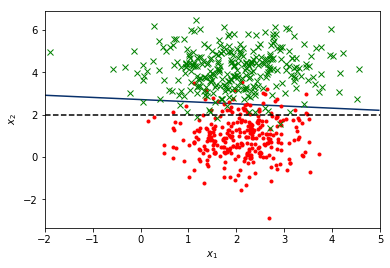
\includegraphics[width=0.49\columnwidth]{biased_boundary.png}
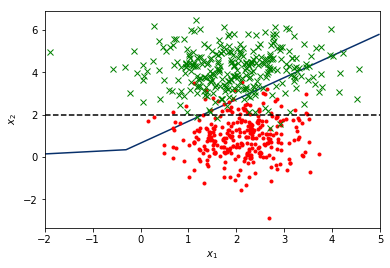
\includegraphics[width=0.49\columnwidth]{debiased_boundary.png}
\caption{Illustrative example to visualize bias reduction with multi-objective learning (Equation \ref{eq:jointloss}). Predictions
with a bias-agnostic classifier (logistic regression with $L_2$ regularization) are effective but exhibits a `bias' in associating the green points with the top half of the plot area (left); whereas the multi-objective learning is able to reduce such a bias (right).
\label{fig:2d-data}}
\end{figure}
\end{frame}
%
\begin{frame}{Evaluation}
%
\begin{table}[t]
\adjustbox{max height=\textheight, max width=\textwidth}{
\centering
\scriptsize
\begin{tabular}{l@{~~}c@{~~}c@{~~}c@{~~}c@{~~}c@{~~}c} 
\toprule
&\multicolumn{5}{c}{Emotion Categories}& \\
\cmidrule(r){2-6}
Identity Attribute &Fear & Anger & Joy & Sadness & Neutral & Total \\
\midrule
Male &1050&	1050&	1050 &	1050&	120	& 4320\\
Female &1050&	1050&	1050 &	1050&	120	& 4320\\
African-American  &700&	700	&700&	700&	120&	2920\\
Caucasian  &700&	700	&700&	700&	120&	2920\\
None  &N/A&	N/A	&N/A&	N/A&	2920 &	2920\\
\midrule
\midrule
\multicolumn{7}{c}{(SS-1): Biased Subsample with (Female, Fear)$\uparrow$, (Male, Anger)$\uparrow$} \\
\midrule
Male &500&	1050&	1050&	1050&	120&	3770\\
Female &1050&	500&	1050&	1050&	120	&3770\\
African-American &450	&550 &	700	&700&	120	&2520\\
Caucasian  &550&	500	&700&700&120&	2570\\
None  &N/A& N/A& N/A & N/A & 1450 & 1450 \\
\midrule
\midrule
\multicolumn{7}{c}{(SS-2): Biased Subsample with (Caucasian, Fear)$\uparrow$} \\
\midrule
Male &850&	1050&	1050&	1050&	120&	3770\\
Female &850&	1050&	1050&	1050&	120	&3770\\
African-American &300	&700 &	700	&700&	120	&2520\\
Caucasian  &700&	700	&700&700&120&	2570\\
None  &N/A& N/A& N/A & N/A & 1450 & 1450 \\
\bottomrule
\end{tabular}
\caption{Fear Distribution }
\label{tab:DataDesc}
\end{table}
}
\end{frame}
%
\begin{frame}{Evaluation}
%
\begin{equation}
U_{x_2}=\{(x_1,x_2) \in \mathbb{R}^2: x_2 > 2\} \label{eq:2dexample}
\end{equation}
\end{frame}
%
\begin{frame}{Evaluation}
%
\begin{equation}
F=\alpha(1-\alpha),\, \alpha=P(y=l|U),
\end{equation}
\end{frame}
%
\begin{frame}{Evaluation}
%
\begin{equation}
\gamma = \frac{AF}{A+F},    
\end{equation}
\end{frame}
%
\begin{frame}{Conclusions and Future Work}
%
\begin{itemize}
\item
In this paper, we propose a multi-objective learning based framework that seeks to effectively learn to predict a primary task (e.g. emotion classification), with an aim to ensure that such predictions do not constitute social prejudices and stereotypes. More specifically, given a set of identity attributes and a set of sensitive categories (primary task labels), our proposed model seeks to reduce certain pairs of associations that are ethically not correct, e.g. predicting that most black-skinned people are prone to be criminals. Our experiments on a dataset of emotion prediction shows that this bias-aware learning framework can reduce a number of different cognitive biases from its predictions, such as reducing the number of times the model predicts an emotion of `fear' for a woman etc. The effectiveness of such an approach could then be evaluated by measuring how well the predictions correlate with unprejudiced human judgments. The first author is supported by Science Foundation Ireland (Grant No.
\end{itemize}
\end{frame}
%
\begin{frame}{Conclusions and Future Work}
%
\begin{table}[t]
\adjustbox{max height=\textheight, max width=\textwidth}{
\footnotesize
\centering
\begin{tabular}{l|c|c|c|c|c|c|c}
\toprule
Method & $Obj$ & $JOBJ$ & Penalty & $Gender$  & Race & $Debiased_Embedding$  \\
\midrule
STWR & \checkmark & \checkmark  &  &  & & & \checkmark &  \\
QFG & \checkmark &   & \checkmark &  & & & & \checkmark \\
QFG + RLM & \checkmark & \checkmark  & \checkmark &  & & & \checkmark & \\
CRLM & \checkmark &   & \checkmark & \checkmark & &\checkmark &\checkmark &  \\
WE & \checkmark &   & \checkmark & \checkmark &\checkmark & &\checkmark &  \\
WET & \checkmark &   & \checkmark & \checkmark &\checkmark &\checkmark &\checkmark &  \\
D2V & \checkmark &   & \checkmark & \checkmark &\checkmark &\checkmark &\checkmark &  \checkmark\\
NMF & \checkmark &   & \checkmark & \checkmark &\checkmark &\checkmark &\checkmark &  \checkmark\\
GRL & \checkmark &   & \checkmark & \checkmark &\checkmark &\checkmark &\checkmark &  \checkmark\\
\bottomrule
\end{tabular}
\caption{A summary of the approaches investigated. The columns denote sources of information, e.g. representation learning (RL), temporal information (T), weighted query (WQ), joint representation (JRL).}
\label{tab:baselines}
\end{table}
}
\end{frame}
%
\end{document}
